\documentclass{article}
\usepackage[a4paper, margin=5em]{geometry}
\usepackage{fancyhdr}
\usepackage{lastpage}
\usepackage{ngerman}
\usepackage{parskip}
\usepackage{hyphenat}
\usepackage{hyperref}
\usepackage{tabularx}
\usepackage{graphicx}
\usepackage{enumitem}
\usepackage{glossaries}
\usepackage[svgnames]{xcolor}

\newcommand{\gqq}[1]{\glqq{}#1\grqq{}}

\pagestyle{fancy}
\fancyhf{}
\renewcommand{\headrulewidth}{0pt}
\fancyfoot{}

\lfoot{}
\cfoot{Seite \thepage\ / \pageref*{LastPage}}
\rfoot{}

\definecolor{fhmint}{RGB}{0,177,172}

\hypersetup{
    colorlinks=true,
    linktoc=all,
    linkcolor=blue
}

\makenoidxglossaries
\newglossaryentry{Betrag}{
    name=Betrag,
    description={Geldwert}
}
\newglossaryentry{Kosten}{
    name=Kosten,
    description={Zu zahlender \gls{Betrag}}
}
\newglossaryentry{Muenzspeicher}{
    name=Münzspeicher,
    description={Gelagerte \gls{Muenzen}}
}
\newglossaryentry{Muenzen}{
    name=Münzen,
    description={Geldwert als rundes Objekt in der Realität}
}
\newglossaryentry{Stakeholder}{
    name=Stakeholder,
    description={\href{https://de.wikipedia.org/wiki/Stakeholder}{Anspruchsberechtigter}}
}
\newglossaryentry{Kunde}{
    name=Kunde,
    description={Zahlungswilliger Kaufinteressierter}
}
\newglossaryentry{Kunden}{
    name=Kunden,
    description={Mehrzahl \gls{Kunde}}
}
\newglossaryentry{Software}{
    name=Software,
    description={Programm und Daten hinter dem Automaten}
}
\newglossaryentry{Benutzeroberflaeche}{
    name=Benutzeroberfläche,
    description={Grafische Schnittstelle von \gls{Kunden} zu dem Automaten}
}
\newglossaryentry{Administration}{
    name=Administration,
    description={Für die \gls{Software} des Systems verantwortliche Verwaltung}
}
\newglossaryentry{Fernwartung}{
    name=Fernwartung,
    description={Wartung aus der ferne}
}
\newglossaryentry{Protokoll}{
    name=Protokoll,
    description={Gespeicherte Beschreibung von Ereignissen mit Zeitstempel und Output}
}
\newglossaryentry{Protokolle}{
    name=Protokolle,
    description={Mehrzahl \gls{Protokoll}}
}
\newglossaryentry{Servicepersonal}{
    name=Servicepersonal,
    description={Für die \gls{Hardware} des Systems verantwortliche Verwaltung}
}
\newglossaryentry{Hardware}{
    name=Hardware,
    description={Physische Komponenten eines Systems}
}
\newglossaryentry{Papier}{
    name=Papier,
    description={Zu beschreibendes Material, welches nach Beschreibung als gültige Fahrberechtigung gewertet wird}
}
\newglossaryentry{Farbbaender}{
    name=Farbbänder,
    description={Material, welches zum beschreiben von \gls{Papier} benötigt wird}
}
\newglossaryentry{Farbbaendern}{
    name=Farbbändern,
    description={Mehrzahl \gls{Farbbaender}}
}
\newglossaryentry{Betriebsmittel}{
    name=Betriebsmittel,
    description={\gls{Papier} und \gls{Farbbaender} sowie \gls{Muenzen}}
}
\newglossaryentry{Betriebsmitteln}{
    name=Betriebsmitteln,
    description={Mehrzahl \gls{Betriebsmittel}}
}
\newglossaryentry{Schaeden}{
    name=Schäden,
    description={Entstandener Geldverlust}
}
\newglossaryentry{Verkehrsbetriebe}{
    name=Verkehrsbetriebe,
    description={Management und Zahlungsgebender hinter dem Automaten; Verwaltende Instanz; Inhaber}
}
\newglossaryentry{Finanzdienstleistende}{
    name=Finanzdienstleistende,
    description={Externe Dienstleistenden für Zahlungen abseits Barzahlung}
}
\newglossaryentry{Zahlungsmethode}{
    name=Zahlungsmethode,
    description={Art der bezahlung; Beispielsweise: Bar, Karte, PayPal, etc \ldots}
}
\newglossaryentry{Zahlungsmethoden}{
    name=Zahlungsmethoden,
    description={Mehrzahl \gls{Zahlungsmethode}}
}
\newglossaryentry{Digitalisierung}{
    name=Digitalisierung,
    description={Seit langem vepasste Chance auf nicht veraltete \gls{Software} und \gls{Hardware} zu setzen}
}
\newglossaryentry{Ticket}{
    name=Ticket,
    description={Fahrkarte}
}
\newglossaryentry{Tickets}{
    name=Tickets,
    description={Mehrzahl \gls{Ticket}}
}
\newglossaryentry{Steuern}{
    name=Steuern,
    description={Öffentliche Abgaben zur Deckung des allgemeinen Finanzbedarfs}
}
\newglossaryentry{Kernaufgabe}{
    name=Kernaufgabe,
    description={Für den Kaufprozess essentielle notwendige Aufgabe}
}
\newglossaryentry{Anzeigesprache}{
    name=Anzeigesprache,
    description={Anzuzeigende Sprache; Beispielsweise: de, en, etc \ldots}
}
\newglossaryentry{Interrupt}{
    name=Interrupt,
    description={Abbruchsgrund mit hoher Priorisierung}
}
\newglossaryentry{ordnungsgemaess}{
    name=ordnungsgemäß,
    description={geplant; korrekt}
}
\newglossaryentry{Ausgangszustand}{
    name=Ausgangszustand,
    description={Zustand nach dem Einschalten des Automaten ohne manipulation Dritter}
}
\newglossaryentry{remote}{
    name=remote,
    description={Aus der ferne; nicht lokal}
}
\newglossaryentry{Service-Account}{
    name=Service-Account,
    description={Ein, nicht zu einem realen Menschen zugeordneter, Benutzer}
}
\newglossaryentry{Service-Accounts}{
    name=Service-Accounts,
    description={Mehrzahl \gls{Service-Account}}
}
\newglossaryentry{Netz}{
    name=Netz,
    description={Verbindung über eine geschützte Verbindung im Internet}
}
\newglossaryentry{Zahlungsschnittstelle}{
    name=Zahlungsschnittstelle,
    description={Schnittstelle, über die gezahlt werden soll}
}
\newglossaryentry{Zahlungsschnittstellen}{
    name=Zahlungsschnittstellen,
    description={Mehrzahl \gls{Zahlungsschnittstelle}}
}

\author{Tim Wende}
\date{\today}
\title{\textbf{Fahrkarten-Automat\\Lastenheft\\(Requirement-Specification)}}

\begin{document}
    \maketitle
    \tableofcontents
    \newpage
    \section{Historie}
    \begin{tabularx}{\textwidth}{|l|l|X|}
        \hline        
        \textbf{Datum} & \textbf{Name} & \textbf{Beschreibung}\\
        \hline
        23.10.2021 & Tim Wende & Erste Version erstellt \\\hline
        23.10.2021 & Tim Wende & \gls{Stakeholder} bestimmt \\\hline
        23.10.2021 & Tim Wende & Ziele formuliert \\\hline
        23.10.2021 & Tim Wende & Anwendungsfalldiagramm erstellt und eingefügt \\\hline
        23.10.2021 & Tim Wende & Anwendungsfälle näher beschrieben \\\hline
        23.10.2021 & Tim Wende & Nichtfunktionale Anforderungen ergänzt \\\hline
        24.10.2021 & Tim Wende & Grafische Oberfläche hinzugefügt \\\hline
    \end{tabularx}

    \section{Stakeholder und Ziele}
    \subsection{\gls{Stakeholder}}
    \begin{itemize}
        \setlength\itemsep{-0.25em}
        \item \nameref{sec:Kunden}
        \item \nameref{sec:Administration}
        \item \nameref{sec:Servicepersonal}
        \item \nameref{sec:Verkehrsbetriebe}
        \item \nameref{sec:Finanzdienstleistende}
    \end{itemize}

    \subsection{Ziele}
    \subsubsection*{Kunden}
    \label{sec:Kunden}
    Zu entwickeln ist die \gls{Software} für einen Fahrkartenautomaten.
    Ein Fahrkartenautomat dient dem Verkauf von Fahrkarten an \gls{Kunden}.
    Dabei soll die \gls{Benutzeroberflaeche} leicht und intuitiv gestaltet sein.
    Der \gls{Kunde} kann den Kaufvorgang jederzeit abbrechen.

    \subsubsection*{Administration}
    \label{sec:Administration}
    Die \gls{Administration} der \gls{Verkehrsbetriebe} kann \gls{remote} auf den Automaten zugreifen.
    Nach erfolgreicher Anmeldung erhalten sie Einsicht über die \gls{Protokolle} sowie den aktuellen \gls{Muenzspeicher} und die \gls{Software}version.
    Zusätzlich soll der Automat via \gls{Fernwartung} deaktiviert werden können.
    Um dies zu erreichen ist der Automat vernetzt mit dem Server der \gls{Verkehrsbetriebe}.
    
    \subsubsection*{Servicepersonal}
    \label{sec:Servicepersonal}
    Sollte die \gls{Administration} feststellen, dass \gls{Papier} oder \gls{Farbbaender} in nicht ausreichender Menge vorhanden sind, soll das Servicepersonal die \gls{Betriebsmittel} regelmäßig nachfüllen können.
    Dieser Auslöser verhindert vermeidbare Laufwege und entlastet somit das \gls{Servicepersonal} ungemein.
    Durch regelmäßige Kontrollen lassen sich ebenfalls unerwünschte Engpässe von \gls{Betriebsmitteln} vermeiden und daraus resultierende \gls{Schaeden} verhindern.

    \subsubsection*{Verkehrsbetriebe}
    \label{sec:Verkehrsbetriebe}
    Da die \gls{Verkehrsbetriebe} die Betreibenden der Automaten sind, wollen sie die \gls{Kosten} dieser möglichst gering halten.
    Somit sollten die Entwicklungs-, Instandhaltungs- sowie Wartungskosten möglichst effizient genutzt werden. 
    Zusätzlich sollte das Produkt eine gute Außenwirkung erziehlen um das Unternehmen positiv zu vermarkten.

    \subsubsection*{Finanzdienstleistende}
    \label{sec:Finanzdienstleistende}
    Die \gls{Finanzdienstleistende} ermöglichen etwaigen \gls{Kunden} umfangreiche \gls{Zahlungsmethoden}.
    Durch diese \gls{Digitalisierung} erweitert sich die Zielgruppe der \gls{Kunden} um solche, die vor allem in Zeiten von Corona ausschließlich kontaktlos bezahlen wollen.
    Im Gegenzug erhalten die Dienstleistenden einen geringen Teil des Gewinns, welcher aus diesen Automaten generiert wird.

    \section{Anwendungsfalldiagramm}
    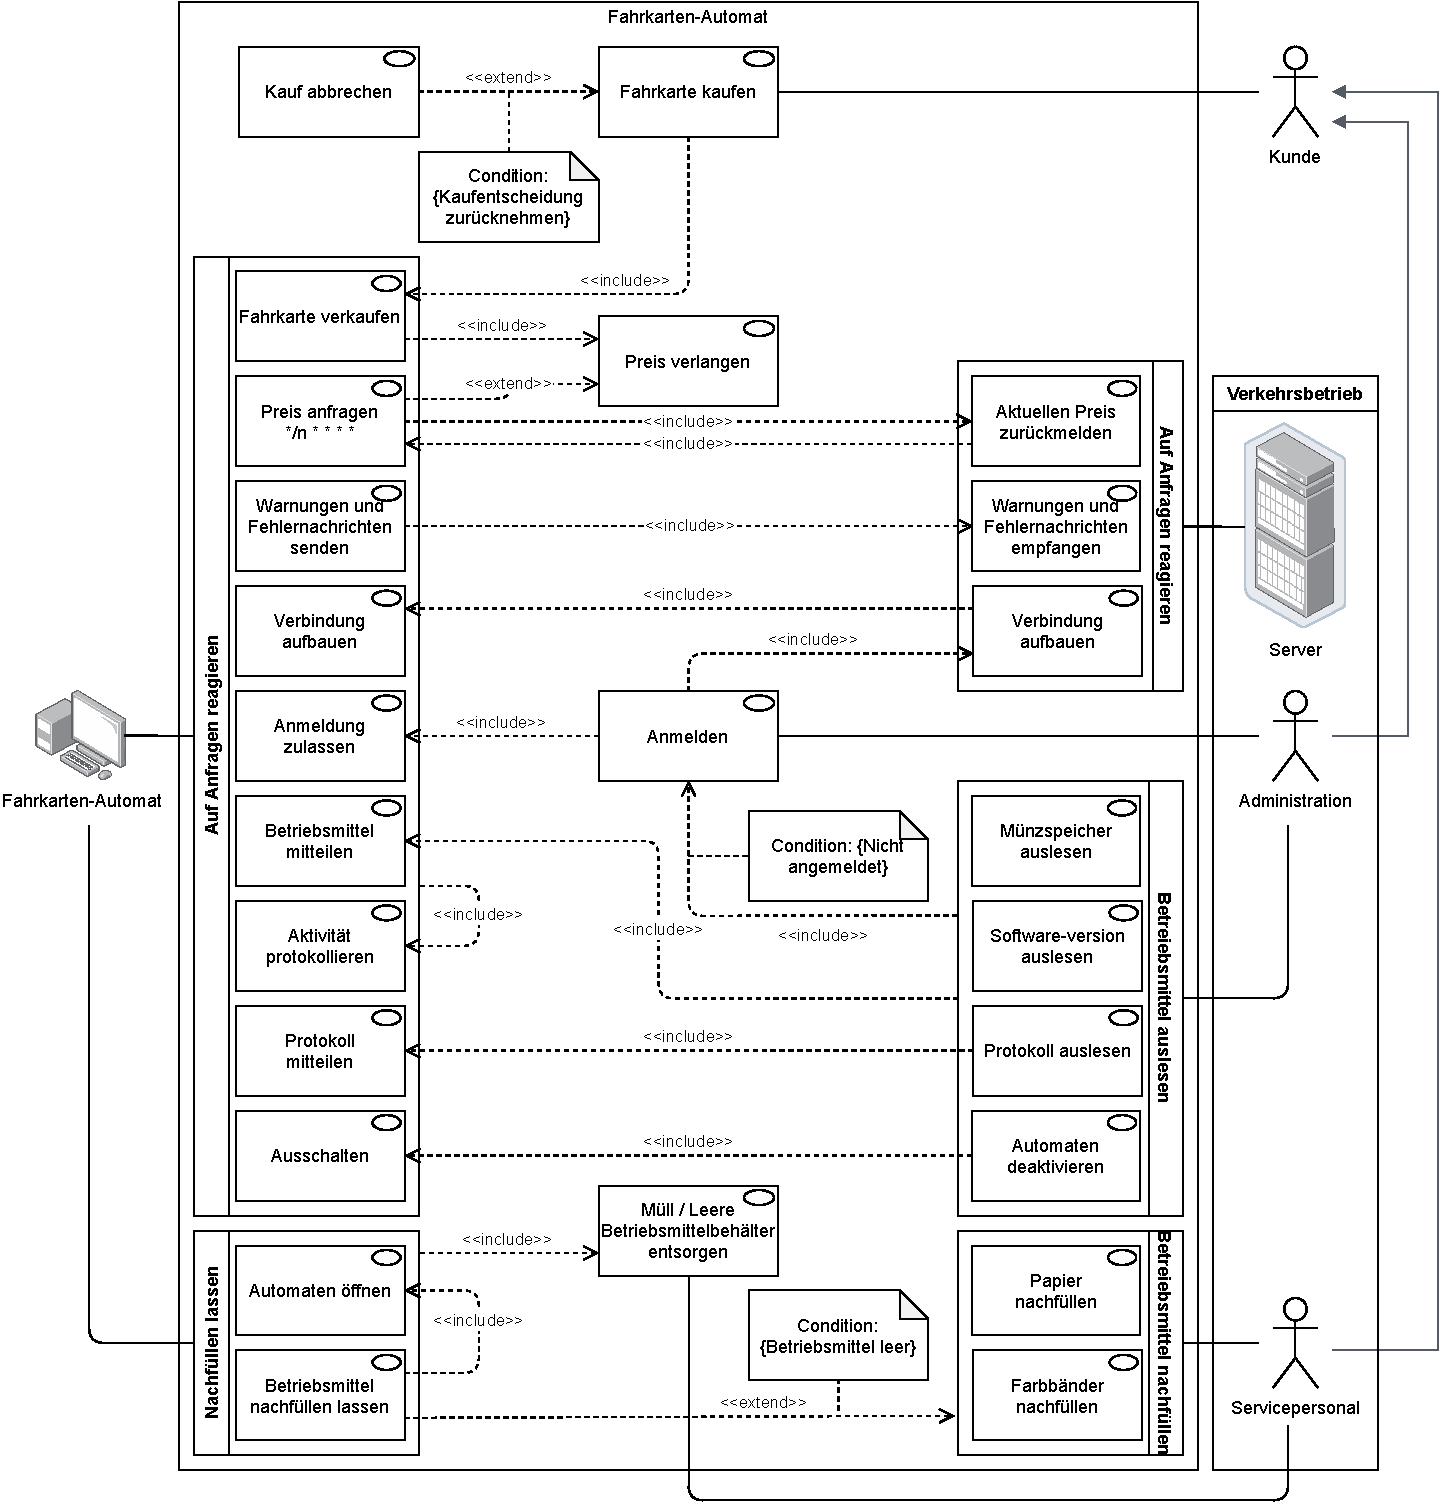
\includegraphics[width=\textwidth]{swt_wende_tim_h03_use_case.pdf}

    \section{Anwendungsfälle}
    \subsection{Fahrkarte kaufen}
    \begin{tabularx}{\textwidth}{|l|X|}
        \hline        
        \textcolor{fhmint}{\textbf{Name des Use Case}} & \LARGE\textcolor{fhmint}{\textbf{Fahrkarte kaufen}}\\
        \hline
        \textbf{Nummer} & UC1 \\\hline
        \textbf{Autor} & Tim Wende \\\hline
        \textbf{Version} & 0.1 Erste Erstellung \\\hline
        \textbf{Kurzbeschreibung} & Der Anwendungsfall beschreibt den den Fahrkartenkauf durch einen Kunden der Verkehrbetriebe \\\hline
        \textbf{beteiligte Aktoren (\gls{Stakeholder})} & \gls{Kunden} \\\hline
        \textbf{Referenzen} & \begin{itemize}
            \item[-] Anzeigen aller verfügbaren \gls{Tickets} in einer übersichtlichen und benutzerfreundlichen grafischen Oberfläche
            \item[-] Abfragen der gewünschten \gls{Zahlungsmethoden}
            \item[-] \gls{Steuern} in den Preis einberechnen
            \item[-] Ändern der \gls{Anzeigesprache}
            \item[-] Aktuelle Angebote anzeigen
        \end{itemize} \\\hline
        \textbf{Vorbedingungen} & \begin{itemize}
            \item Fahrkartenautomat arbeitet \gls{ordnungsgemaess}
            \item Preis von dem Automaten bereits angefragt
            \item Automat verfügt über ein passendes \gls{Ticket}
            \item \gls{Kunde} hat genügend Geld
        \end{itemize} \\\hline
        \textbf{Nachbedingungen} & \begin{itemize}
            \item Fahrkarte von dem Automaten verkauft
            \item Preis von dem Automaten verlangt
            \item Rückgeld korrekt zurückgezahlt
        \end{itemize} \\\hline
        \textbf{typischer Ablauf} & \begin{enumerate}
            \item Ein \gls{Kunde} startet an einem Automaten den Kaufvorgang
            \item Dieser wird an den Automaten weitergegeben
            \item Des Weiteren berechnet der Automat den Preis
            \item Dieser wird von dem \gls{Kunden} bezahlt
            \item Zum Schluss druckt der Automat das passende \gls{Ticket}
        \end{enumerate} \\\hline
        \textbf{alternative Abläufe} & \begin{itemize}
            \item \begin{enumerate}
                \item Ein \gls{Kunde} startet an einem Automaten den Kaufvorgang
                \item Der \gls{Kunde} findet jedoch kein passendes \gls{Ticket}
                \item Daraufhin wird der Kauf abgebrochen
            \end{enumerate}
            \item \begin{enumerate}
                \item Ein \gls{Kunde} startet an einem Automaten den Kaufvorgang
                \item Dieser wird an den Automaten weitergegeben
                \item Des Weiteren berechnet der Automat den Preis
                \item Der \gls{Kunde} bemerkt, dass er nicht genug Geld hat
                \item Daraufhin wird der Kauf abgebrochen
                \item Zum Schluss beendet der Automat die offene Zahlung
            \end{enumerate}
        \end{itemize} \\\hline
        \textbf{Kritikalität} & \gls{Kernaufgabe} des Automaten \\\hline
        \textbf{Verknüpfungen} & UC2 Fahrkarte verkaufen \\\hline
        \textbf{funktionale Anforderungen} & siehe Text. \\ 
        & E: Gewünschtes \gls{Ticket} \\
        & E: Start und Zielort \\
        & A: Zu zahlendes Geld \\
        & E: Geld (bar / kontaktlos) \\
        & A: \gls{Ticket} \\
        & A: Rückgeld \\\hline
        \textbf{nicht funktionale Anforderungen} & \begin{itemize}
            \item[-] Möglichkeiten zum Anpassen der \gls{Anzeigesprache}
            \item[-] Nächtliches Design zum Sparen von Energie
            \item[-] Implementierung verschiedenster \gls{Zahlungsmethoden}
            \item[-] Implementierung verschiedenster \gls{Zahlungsschnittstellen}  
        \end{itemize} \\\hline
    \end{tabularx}

    \subsection{Kauf abbrechen}
    \begin{tabularx}{\textwidth}{|l|X|}
        \hline        
        \textcolor{fhmint}{\textbf{Name des Use Case}} & \LARGE\textcolor{fhmint}{\textbf{Kauf abbrechen}}\\
        \hline
        \textbf{Nummer} & UC3 \\\hline
        \textbf{Autor} & Tim Wende \\\hline
        \textbf{Version} & 0.1 Erste Erstellung \\\hline
        \textbf{Kurzbeschreibung} & Der Anwendungsfall beschreibt den Abbruch des Kaufes eines \gls{Tickets} \\\hline
        \textbf{beteiligte Aktoren (\gls{Stakeholder})} & \gls{Kunden} \\\hline
        \textbf{Referenzen} & \begin{itemize}
            \item[-] Soll als \gls{Interrupt} immer zur Verfügung stehen
        \end{itemize} \\\hline
        \textbf{Vorbedingungen} & \begin{itemize}
            \item Fahrkartenautomat arbeitet \gls{ordnungsgemaess}
            \item Laufender Kauf in Gange
        \end{itemize} \\\hline
        \textbf{Nachbedingungen} & \begin{itemize}
            \item Automat in \gls{Ausgangszustand} versetzen
        \end{itemize} \\\hline
        \textbf{typischer Ablauf} & \begin{enumerate}
            \item Ein \gls{Kunde} startet an einem Automaten den Kaufvorgang
            \item Dieser wird an den Automaten weitergegeben
            \item Des Weiteren berechnet der Automat den Preis
            \item Der \gls{Kunde} bemerkt, dass er nicht genug Geld hat
            \item Daraufhin wird der Kauf abgebrochen
            \item Zum Schluss beendet der Automat die offene Zahlung
        \end{enumerate} \\\hline
        \textbf{alternative Abläufe} & \begin{itemize}
            \item \begin{enumerate}
                \item Ein \gls{Kunde} startet an einem Automaten den Kaufvorgang
                \item Der \gls{Kunde} findet jedoch kein passendes \gls{Ticket}
                \item Daraufhin wird der Kauf abgebrochen
            \end{enumerate}
        \end{itemize} \\\hline
    \end{tabularx}

    \subsection{Anmelden}
    \begin{tabularx}{\textwidth}{|l|X|}
        \hline        
        \textcolor{fhmint}{\textbf{Name des Use Case}} & \LARGE\textcolor{fhmint}{\textbf{Anmelden}}\\
        \hline
        \textbf{Nummer} & UC4 \\\hline
        \textbf{Autor} & Tim Wende \\\hline
        \textbf{Version} & 0.1 Erste Erstellung \\\hline
        \textbf{Kurzbeschreibung} & Der Anwendungsfall beschreibt die Anmeldung am Automaten \\\hline
        \textbf{beteiligte Aktoren (\gls{Stakeholder})} & \gls{Administration} \\\hline
        \textbf{Referenzen} & \begin{itemize}
            \item[-] Ist Bedingung den Automaten \gls{remote} zu konfigurieren
            \item[-] \gls{Service-Accounts} sollen zur Verfügung gestellt werden können
        \end{itemize} \\\hline
        \textbf{Vorbedingungen} & \begin{itemize}
            \item Fahrkartenautomat arbeitet \gls{ordnungsgemaess}
            \item Anmeldedaten vorhanden
        \end{itemize} \\\hline
        \textbf{Nachbedingungen} & \begin{itemize}
            \item Verbindung zum Automaten vorhanden
        \end{itemize} \\\hline
        \textbf{typischer Ablauf} & \begin{enumerate}
            \item Der \gls{Kunde} meldet sich über das Verkehrsbetrieb-interne \gls{Netz} am Fahrkarten-Automaten an
            \item Auf der Anmeldeseite gibt der Administrierende sein Benutzernamen sowie Passwort ein
        \end{enumerate} \\\hline
        \textbf{alternative Abläufe} & \begin{itemize}
            \item \begin{enumerate}
                \item Der \gls{Kunde} meldet sich über das Verkehrsbetrieb-interne \gls{Netz} am Fahrkarten-Automaten an
                \item Auf der Anmeldeseite gibt der Administrierende die Anmeldedaten des ihm zur Verfügung gestellten \gls{Service-Accounts} ein
            \end{enumerate}
        \end{itemize} \\\hline
    \end{tabularx}

    \subsection{\gls{Farbbaender} nachfüllen}
    \begin{tabularx}{\textwidth}{|l|X|}
        \hline        
        \textcolor{fhmint}{\textbf{Name des Use Case}} & \LARGE\textcolor{fhmint}{\textbf{\gls{Farbbaender} nachfüllen}}\\
        \hline
        \textbf{Nummer} & UC5 \\\hline
        \textbf{Paket}
        \textbf{Autor} & Tim Wende \\\hline
        \textbf{Version} & 0.1 Erste Erstellung \\\hline
        \textbf{Kurzbeschreibung} & Der Anwendungsfall beschreibt den Austausch der \gls{Farbbaender} \\\hline
        \textbf{beteiligte Aktoren (\gls{Stakeholder})} & \gls{Servicepersonal} \\\hline
        \textbf{Referenzen} & \begin{itemize}
            \item[-] Ohne Farbe auf den \gls{Farbbaendern} kann der Automat keine \gls{Tickets} drucken.
                Somit ist dies eine sehr relevante Aufgabe in dem Prozess 
        \end{itemize} \\\hline
        \textbf{Vorbedingungen} & \begin{itemize}
            \item {Farbbaender} leer
        \end{itemize} \\\hline
        \textbf{Nachbedingungen} & \begin{itemize}
            \item Neues Farbband besorgen
            \item Leeres Farbband entsorgen
        \end{itemize} \\\hline
        \textbf{typischer Ablauf} & \begin{enumerate}
            \item Die Servicekraft öffnet den Automaten
            \item Das leere Farbband wird entfernt
            \item Das neue Farbband wird an den dafür vorgesehenen Platz gesetzt
            \item Der Automat wird von der Servicekraft geschlossen
            \item Der Automat erkennt die veränderte \gls{Hardware} und loggt dieses
        \end{enumerate} \\\hline
        \textbf{alternative Abläufe} & \begin{itemize}
            \item \begin{enumerate}
                \item Die Servicekraft öffnet den Automaten
                \item Das leere Farbband wird entfernt
                \item Es wird ein inkompatibles Farbband gewählt
                \item Dadurch kann der Drucker nicht drucken und
                \item ein Fehler wird an den Server gemeldet
            \end{enumerate}
        \end{itemize} \\\hline
    \end{tabularx}

    \section{Nichtfunktionale Anforderungen}
    \begin{enumerate}[font={\bfseries}, label={NFRQ\arabic*:}]
        \setlength\itemsep{-0.25em}
        \item Möglichkeiten zum Anpassen der \gls{Anzeigesprache}
        \item Implementierung verschiedenster \gls{Zahlungsmethoden}
        \item Implementierung verschiedenster \gls{Zahlungsschnittstellen}
        \item Adminstrative grafische \gls{Benutzeroberflaeche}:
    \end{enumerate}
    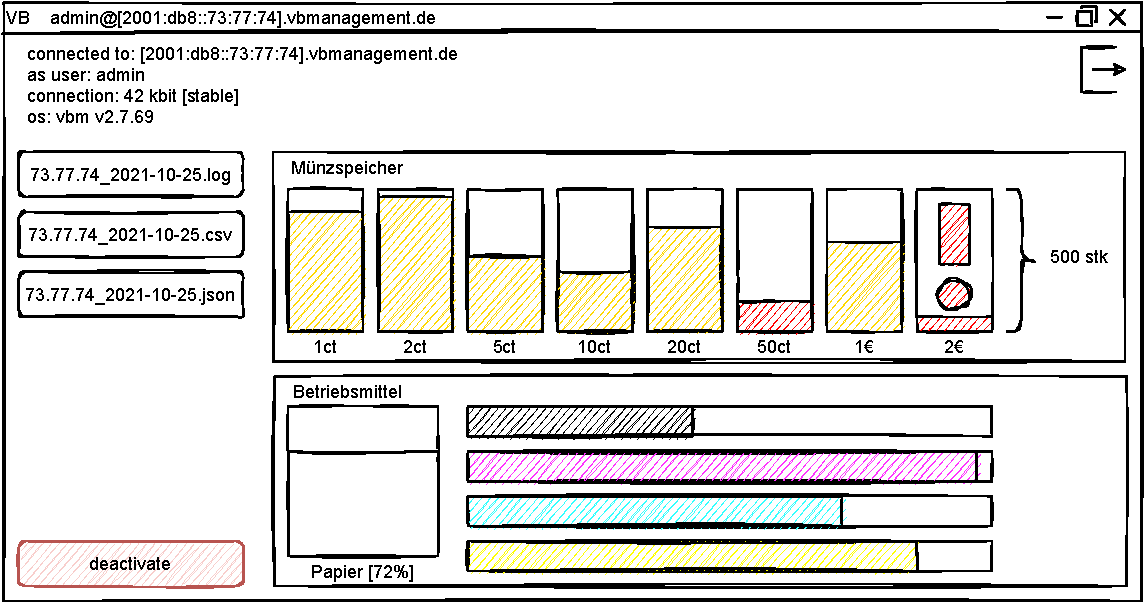
\includegraphics[width=\textwidth]{swt_wende_tim_h03_gui.pdf}

    \clearpage
    \printnoidxglossaries
    \addcontentsline{toc}{section}{Glossar}
\end{document}